\documentclass[12pt,a4paper]{article}
\usepackage[utf8]{inputenc}
\usepackage[T1]{fontenc}
\usepackage{amsmath}
\usepackage{amsfonts}
\usepackage{amssymb}
\usepackage{graphicx}
\author{Evren Turan}
\title{Growth Curves}
\usepackage{subcaption}
\usepackage{tikz}
\usepackage{pgfplots}
\usepackage[style=authoryear-comp]{biblatex}
\addbibresource{Bib.bib}
\begin{document}
	\section*{Growth curves: Regression and ranking of growth curves}
	\section{Introduction}
	Growth curves are widely used to model animal growth. In general experimental data of a population is gathered and growth curves are fitted to the samples and one is chosen to represent the growth of the population. These curves are generally sigmoidal or attenuating, and common models include the logistic, Gompertz, and von Bertalanffy curves, as shown in Table \ref{tab:Popularity of curves}.
	
	Typically there are many different parametrisations of these curves, for example see \textcite{Tjorve2010} which compares the different different parametrisations of the Richards curve. These different parametrisations result in mathematically equivalent forms, yet due to the nature of the numerical algorithms different parametrisations may work better for different data sets \textcite{Myhrvold2013}.
	\section{Literature}
	\subsection{Regression of growth curves}
	
		\begin{table}[h]
		\centering
		\begin{tabular}{l r}
			\hline
			Model name & Number of results \\
			\hline
			Logistic&3908\\
			Gompertz & 1566\\
			Von Bertalanffy&1477\\
			Richards       & 593\\
			Weibull&591\\
			Michaelis-Menten&179\\
			Monomolecular&129\\
			He Legendre&88\\
			Korf&39\\
			Morgan-Mercer-Flodin & 16\\
			Levakovic&6\\
			\hline
		\end{tabular}
		\caption{Number of results according to web of science search across all databases, including the model name and the phrase "growth curve"}\label{tab:Popularity of curves}
	\end{table}
	Various mathematical models can be used to explain and interpret growth. Asymptotic models (often sigmoidal) are commonly used to describe determinate growth, while a wide range of models can be used for indeterminate growth. Models are commonly written in algebraic form although differential models do exist, for examples see \textcite{Myhrvold2013,Brunner2019}. Models in differential form can sometimes be more flexible however they are more difficult to regress to data sets, in this paper only models that can be written in closed algebraic forms will be considered.
	
	
	Despite the number of available models one commonly finds works in which very few models are compared to each other, typically less than three: for example 
	\begin{table}
	\centering
	\begin{tabular}{l r}
		\hline
		Paper & Number of Models \\
		\hline
		\textcite{Myhrvold2013}&77 \\
		\textcite{Do2019}&10\\
		\textcite{Garcia-Muniz2019}&10  \\ % check, may have been 6
		\textcite{GhaviHossein-Zadeh2015} & 5\\
		\textcite{Kheirabadi2019} & 5\\
		\textcite{Cooper2008}&5\\
		\textcite{Gbangboche2008}&4\\
		\textcite{Araujo2012}&4\\
		\textcite{Keskin2009} &4\\
		\textcite{Perotto1992}&4\\
		\textcite{Xie2020}&3\\
		\textcite{Erickson2015}&3  \\
		\textcite{DeNise1985} &2\\
		\textcite{Waheed2011}&2\\
		\textcite{Yakupoglu2001}&2\\
		\textcite{Ersoy2006}&1 \\
		\textcite{Bathaei1998}&1 \\
		\textcite{Raji2014}&1\\
		\textcite{Ghiasi2018}&1\\
		\textcite{Li2019}&1\\
		\textcite{Lehman2008}&1\\
		\textcite{Chinsamy1990}&1\\
		\hline
	\end{tabular}
	\caption{The number of growth curves compared in various papers}
		\end{table}
	\subsubsection{Uncertainty in one variable}
	The determination of growth curves parameters is an example of explicit regression, i.,e.
	\begin{equation}
	y \approx f(x:\beta)
	\end{equation}
	Where $y$ is the growth variable (size, length, etc.), $x$ is the time variable, and $\beta$ is the vector of fitted parameters. $y$ is only approximately equal to $f(x)$ due to uncertainty (unknown errors) in $x$ and or $y$. For a sample $i$ from the population, the exact equation is written as:
	\begin{equation}
	y_i = f(x_i+\delta_i:\beta)+\epsilon_i
	\end{equation}
	With $\delta_i$ is the error in $x$, $\epsilon$ is the error in $y$ and the subscript $i$ refers to the specific sample. These errors are assumed to be normally distributed and independent.
	
	If there are significant errors in only the $y$ variable, i.e. $\delta_i=0$ for any $i$, then ordinary least squares (OLS) can be used to perform the regression. 	This is because a key assumption of OLS is that the measurements of the independent variable ($x$, age)  are without errors. If the  $x$ variable has errors then it is fundamentally flawed to use OLS. 
	
	Depending on how the samples are taken there may be errors in the ages of the animal --- this is typically the case when feral animals are being sampled and the age is estimated by features of the animal for example see \textcite{Mayberry2018}. Commonly the growth variable ($y$) can be accurately measured (e.g. in the case of weight), which means that there would still be error in only one of the variables. The growth function ($f$) can be inverted ($f^-1=g$) and OLS can be used with $y_i$ as the independent variable, i.e. 
	\begin{equation}
	x_i = g(y_i:\beta)+\epsilon_i
	\end{equation}
	This method of inversion to use OLS is referred to as inverted OLS (OLSI) in this work. This method measures the residuals in a fundamentally different way, shown graphically in Figure \ref{fig:Regression_error_direction}. The variable which has no measurement error is assumed to be exact and the residual is measured as occurring entirely in the other variable. Thus the use of OLSI can give different regressed parameters to OLS.
	
	The use of OLSI has been recommended numerous times over the years \parencite{Myhrvold2013,Kaufmann1981}, yet it is common find that it is not specified if inverted functions are used, or to examine the methodology and see the use of non-inverted functions despite errors in the age variables, for example \textcite{Erickson2015}.
	
	Although the inversion of the growth curve functions is typically simple, using inverted functions does result in different restrictions in the variables, i.e. the function $g$ must accept any of the population sample $y$ values, while $f$ must accept any of the $x$ values. To give an example, the logistic curve is given by:
	
	\begin{align}
		y &= f(x) = \frac{a}{1+e^{-b(-c+x)})} \qquad a>0,\quad b>0\\
		x &= g(y) = \frac{bc-\ln(-1+\frac{a}{y})}{b} \qquad a>y,\quad b>0
	\end{align}
	
	One cannot take the natural log of 0 and hence the inversion of $f$ introduces a constraint that was not present in the un-inverted form.
	
	\subsubsection{Uncertainty in two variables}
	If there is significant uncertainty in both the $x$ and $y$ values of the sample then an error-in-variable regression model must be used. A commonly used model is orthogonal distance regression (ODR). 
	
	Graphically, in ODR the error of the fit by a line orthogonal to the curve, shown in Figure \ref{fig:Regression_error_direction}. A robust, and widely used implementation of ODR, was introduced by \textcite{Boggs1989}, updated in \textcite{Zwolak2007}. This algorithm is available in various programming languages including Python and R. 	One should weight the errors in the different variables, typically by the estimated variance in the parameters.
	
	This method along with OLS and OLSI is used in this work, when appropriate.
	
	\begin{figure}
		\centering
		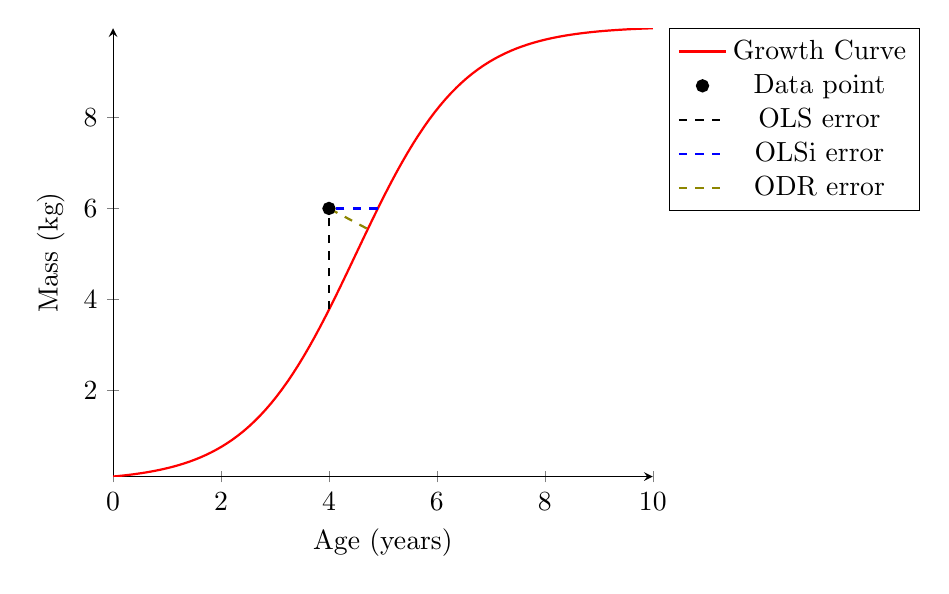
\begin{tikzpicture}
		\begin{axis}[
		axis lines = left,
		xlabel = Age (years),
		ylabel = Mass (kg),
		legend pos=outer north east,
		every axis plot/.append style={ thick},
		]
		%Below the red parabola is defined
		\addplot [
		domain=0:10, 
		samples=100, 
		color=red,
		]
		{10/(1+exp(-1*(-4.5+x)))};

		\addlegendentry{Growth Curve}
		\addplot[only marks,mark=*] coordinates{
			(4,6)
		};
		\addlegendentry{Data point}
		\addplot[black,dashed] coordinates{
			(4,3.78)
			(4,6)
		};
		\addplot[blue,dashed] coordinates{
		(4.9,6)
		(4,6)
		};
		\addplot[olive,dashed] coordinates{
		(4.7,5.56)
		(4,6)
		};
		\addlegendentry{OLS error}
		\addlegendentry{OLSi error}
		\addlegendentry{ODR error}
		\end{axis}
		\end{tikzpicture}
		\caption{Example of the different measurements of fit according to OLS, OLSi and ODR. The growth curve is a logistic curve, with $a=10$, $b=-1$ and $c=-4.5$}\label{fig:Regression_error_direction}
	\end{figure}

	\subsection{Criteria for model selection}
	Once the growth curve parameters have been fitted, one must select a model(s) that best describes the data. Although this has been been done by "author judgement" there are statistical parameters that give indications how well the models fit the data.
	
	\subsubsection{The coefficient of determination}
	The most common widely used parameter is the coefficient of determination ($R^2$). This is the proportion of variance in the dependent variable predicted from the independent variable. The best possible value of $R^2$ is 1, which indicates the model exactly fits the data, with worse models having a lower value.
	
	\begin{align}
	R^2 &= 1- \frac{RSS}{TSS}
	\end{align}
	where RSS is the residual sum of squares and TSS is the total sum of squares.
	
	It is important to note that $R^2$ gives no measure of over-fitting, and that increasing the number of parameters in a model will always increase $R^2$ or keep it constant. 
	


	\subsubsection{Information Criterions}
	The Akaike information criterion (AIC) is an estimator of the quality of a model and is commonly used to give a statistical basis of model selection \parencite{Akaike1974}. An alternative criterion that is widely used is the Bayesian  information criterion (BIC), also known as the Schwarz information criterion  \parencite{Schwarz1978}. With both criterions the "preferred" model has the lowest value. Both of the criterions are similar measures the goodness of model fit and penalise it according to the number of model parameters. This can be interpreted as an implementation of Occam's Razor, i.e. for models that are similar in accuracy, the simpler model (i.e. has less adjustable parameters) is the better choice. 	The criterions are defined as:
	\begin{align}
	AIC &= 2k - 2\ln (L)\\
	BIC &= k\ln(n) - 2\ln (L) \\
	-2\ln(L) &=  n\ln \frac{RSS}{n}
	\end{align}
	where $RSS$ is the residual sum of squares, $n$ is the number of samples, $k$ is the number of parameters, $L$ is the maximum value of the likelihood functions. 
	
	Note that errors are assumed to be independent and identically distributed with zero mean, which specifies the variance of the error which contributes to the count of parameters, $k$. To give an example: a linear fit,
	\begin{equation}
		y\approx\beta_o+\beta_1x
	\end{equation}
	has $k=3$ if there are errors in one variable, and $k=4$ if there are errors in both variables.
	
	As the the information criterions are used to compare models it is common practice to calculate them as $\Delta$ values, i.e.
	\begin{equation}
	\Delta IC_k = IC_k - \min(IC) 
	\end{equation}
	where $IC$ is some information criterion, $\min(IC)$ is the minimum criterion found, and the subscript $k$ refers to a particular model. For example if one was comparing models, $M_1$ and $M_2$ with AIC's of 10 and 12 respectively then the $\Delta$AIC's are 0 and 2. 
	
	Both criterions may may select models incorrect models when small data sets are used: AIC tends to select models that over-fit while BIC selects those that under-fit \parencite{Hurvich1989,McQuarrie1999}. Corrections can be defined to correct for this behaviour, giving the corrected AIC (AICc) and BIC (BICc):
	
	\begin{align}
		AICc &= AIC + \frac{2k(k+1)}{n-k-1}\\
		BICc &= k\ln(n)\frac{n}{n-k-1} - 2\ln (L) 
	\end{align}
	
	Both of the correction converge to the uncorrected criterion when the number of samples is large, and their use is commonly advised over the uncorrected samples \parencite{Burnham2002}.
	\subsubsection{Interpreting the criterions}
	
	
	If there is a "true model" is in the set of available models then BIC will select the true model with 100\% probability, as  $n \rightarrow \infty$. A "true model" is the model that generates the data. The existence of such a "true model" when using real data is questionable. It was famously noted "All models are wrong" \parencite{Box1976}, or to be more explicit, it is unlikely that any real system can be described exactly by some simple model.
	
	There is no guaranteed that AIC will select the "true model" as it may select a more complex, but better fitting, wrong model \parencite{Burnham2002}. As growth is unlikely to be governed exactly by any growth model, the use of BIC doesn't hold any advantage over AIC. Some authors strongly suggest that AIC should be used over BIC, while others recommend reporting both \parencite{Burnham2011,AndrewH.2013}. Both AIC, BIC and their corrected forms are calculated in this paper.
	
	
	Plausible models are generally taken as having a $\Delta AICc\leq4$, with implausible models having $\Delta AICc>14$ \parencite{Burnham2011}. The exact cut-off value to not consider a model varies, with some recommending that models up to $\Delta=7$ should be considered.
\section{Case studies}
\subsection{How the choice of regression method changes parameters}
Data for the ceratopsian dinosaur \emph{Psittacosaurus lujiatunensis} is given in \textcite{Erickson2015,Erickson2009}. Femoral lengths and growth lines were used to estimate specimen mass and age respectively, with data shown in Table \ref{tab:Growth_data_dino}. Mass estimates were used to compare the growth curve to other dinosaurs and living vertebrates \textcite{Erickson2015}. Three growth curves were computed and a logistic curve was chosen based on its $R^2$ value, and because the Gompertz curve was "biologically unreasonable". Issues with the methodology have been raised by Myhrvold, \parencite{Myhrvold2015,Myhrvold2013}, leading to a later response by the original authors in \textcite{Erickson2015}. These issues will not be delved into here, instead the focus is on the choice of regression method, and what impact this has on the regression. Table \ref{tab:Growth_data_dino} clearly shows that there is (large) age estimation, as age is approximated from growth lines, some of which are destroyed. The uncertainty in the femoral length measurements is marginal in comparison. Thus it would be justifiable to perform inverse OLS (OLSi) as discussed above and in \textcite{Kaufmann1981}. 
 
 
\begin{table}
	\centering
	\begin{tabular}{r r r r}
		\hline
		Femoral length (mm) & Growth lines  & Age estimate (years) & Mass estimation\\
		\hline
		49-55 & 0 & 0.5 & 0.45\\
		49-55 & 0 & 0.5 & 0.45\\
		34 & 1 & 1 & 0.12\\ 
		38-45 & 1 &1& 0.29\\
		52 & 2 & 2 &0.50\\
		80-85 & 3 &3&1.61\\
		80-83 &3-4 &3&1.97\\
		103 & 2 & 3 &3.50\\
		101-105 & 2-3 & 4&3.30\\
		95-98 &  3-4 & 4&3.01\\
		108-112 & 3-4&5&4.02\\
		110-111 & 4 & 5&4.34\\
		135-144 & 5 & 7&8.40\\
		149-150&4&7&7.87\\
		135-137&5-6&7&8.05\\
		135 & 5 &7&10.80\\
		164-165&6-7&8&10.36\\
		153-156&5&8&11.97\\
		148&5-7&8&14.36\\
		189-190&7-8&9&21.94\\
		199-201&8&10&25.96\\
		200-202&6&11&25.96\\
		
		\hline
	\end{tabular}
	\caption{Growth data of \emph{Psittacosaurus lujiatunensis} from \textcite{Erickson2015}}\label{tab:Growth_data_dino}
\end{table}

\textcite{Erickson2015} chose the three parameter logistic function:
\begin{equation}\label{eq:logistic}
y = \frac{a}{1+\exp{-b(x-c)}}
\end{equation}
with parameter values of $a=37.48$, $b=0.55$ and $c=9.03$. The uncertainties in these parameters were not given so the developed code was used to perform OLS followed by OLSi regression and these results are presented in Table \ref{tab:OLS_vs_OLSi}.

Based on the results, it is clear that \textcite{Erickson2015} used the OLS method as the fitted parameters (Table \ref{tab:OLS_vs_OLSi}) are exactly as reported. OLSi and OLS give different nominal parameters (i.e. central parameters in the confidence range), with OLSi giving smaller ranges for the parameters. This is most noticeable in the $a$ parameter in which the parameter decreases by nearly half. 

Thus the use of the OLSi and OLS on this data will give different curves, as shown in Figure \ref{fig:fig}, due to the differences in nominal values and uncertainties. Although the shape of the curve is similar there are striking differences in the confidence band. This is expected, as the methods differ based on to which variable the “fitting error” is associated with. The figure clearly shows the influence that the choice of regression method can have, as interpretation of the growth curves would differ, with regression with mass as the independent variable being statistically advised \parencite{Kaufmann1981,Myhrvold2013}. Note that the large uncertainty near the asymptote is simplyu due to the lack of data points above 13 years. 

\begin{table}
	\centering
	\begin{tabular}{l c c}
		\hline
		Parameter & OLS  & OLSi \\
		\hline
		a & 37.48 $\pm$ 6.48 & 31.26 $\pm$ 3.67\\
		b & 0.55 $\pm$ 0.08 & 0.63 $\pm$ 0.05\\
		c & 9.03 $\pm$ 0.72 & 8.04 $\pm$ 0.56\\
		\hline
	\end{tabular}
	\caption{Fitted parameters for the \emph{Psittacosaurus lujiatunensis} data, using inverted and normal OLS with Equation \ref{eq:logistic}}\label{tab:OLS_vs_OLSi}
\end{table}


\begin{figure}[ht]
	\begin{subfigure}{.5\textwidth}
		\centering
		% include first image
	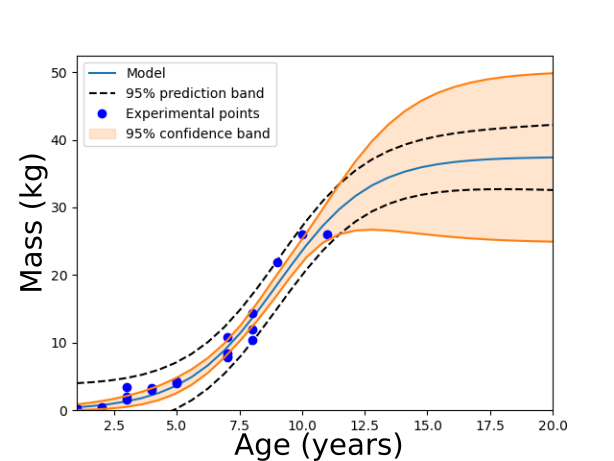
\includegraphics[width=1.0\linewidth]{gfx/Dino_ex1_ols/OLS}
		\caption{Age as independent variable (OLS)}
		\label{fig:sub-first}
	\end{subfigure}
	\begin{subfigure}{.5\textwidth}
		\centering
		% include second image
	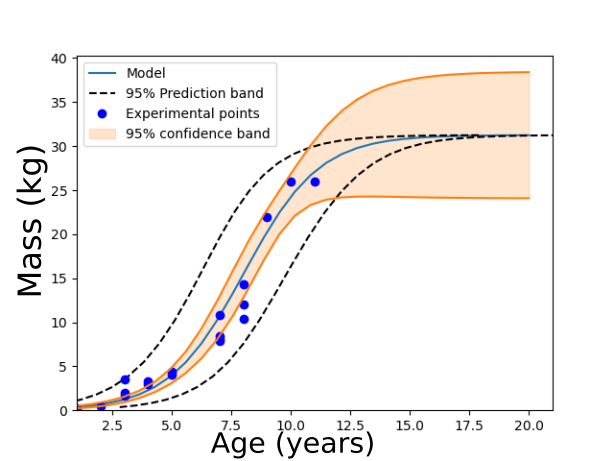
\includegraphics[width=1.0\linewidth]{gfx/Dino_ex1_ols/inverse}
		\caption{Mass as independent variable (iOLS)}
		\label{fig:sub-second}
	\end{subfigure}
	\caption{Comparison of choice of independent variable for the \emph{Psittacosaurus lujiatunensis} data}
	\label{fig:fig}
\end{figure}


\end{document}